\newpage
\section{Exploration}

\subsection{Initial Trials}

With the aim of understanding how the number of rounds affects the orderedness of the cards in play, I first collected data on the relationship between the following variables:

\begin{table}[H]
\centering
\begin{tabular}{lll}
\toprule
Axis & Description & Variable \\
\midrule
$x$ & The number of rounds played & Independent \\
$y$ & The cards flipped from the draw pile & Dependent \\
\bottomrule	
\end{tabular}
%TODO write this caption
\caption{Variables for first investigation}
\label{tb:variables}
\end{table}

 The cards flipped from the draw pile is a key indicator that isolates the orderedness of only the cards in play rather than assessing the orderedness of the whole deck. At this stage, I thought this would reduce the scope and therefore the complexity of the data.
 However, after collecting this data and graphing it on Desmos, I discovered that the relationship gave a random result that didn't indicate any kind of trend, like the one I had hypothesised.
 
  \begin{figure}[H]
	\begin{minipage}[t]{0.48\textwidth} % First image takes up 48% of the width
        \centering
        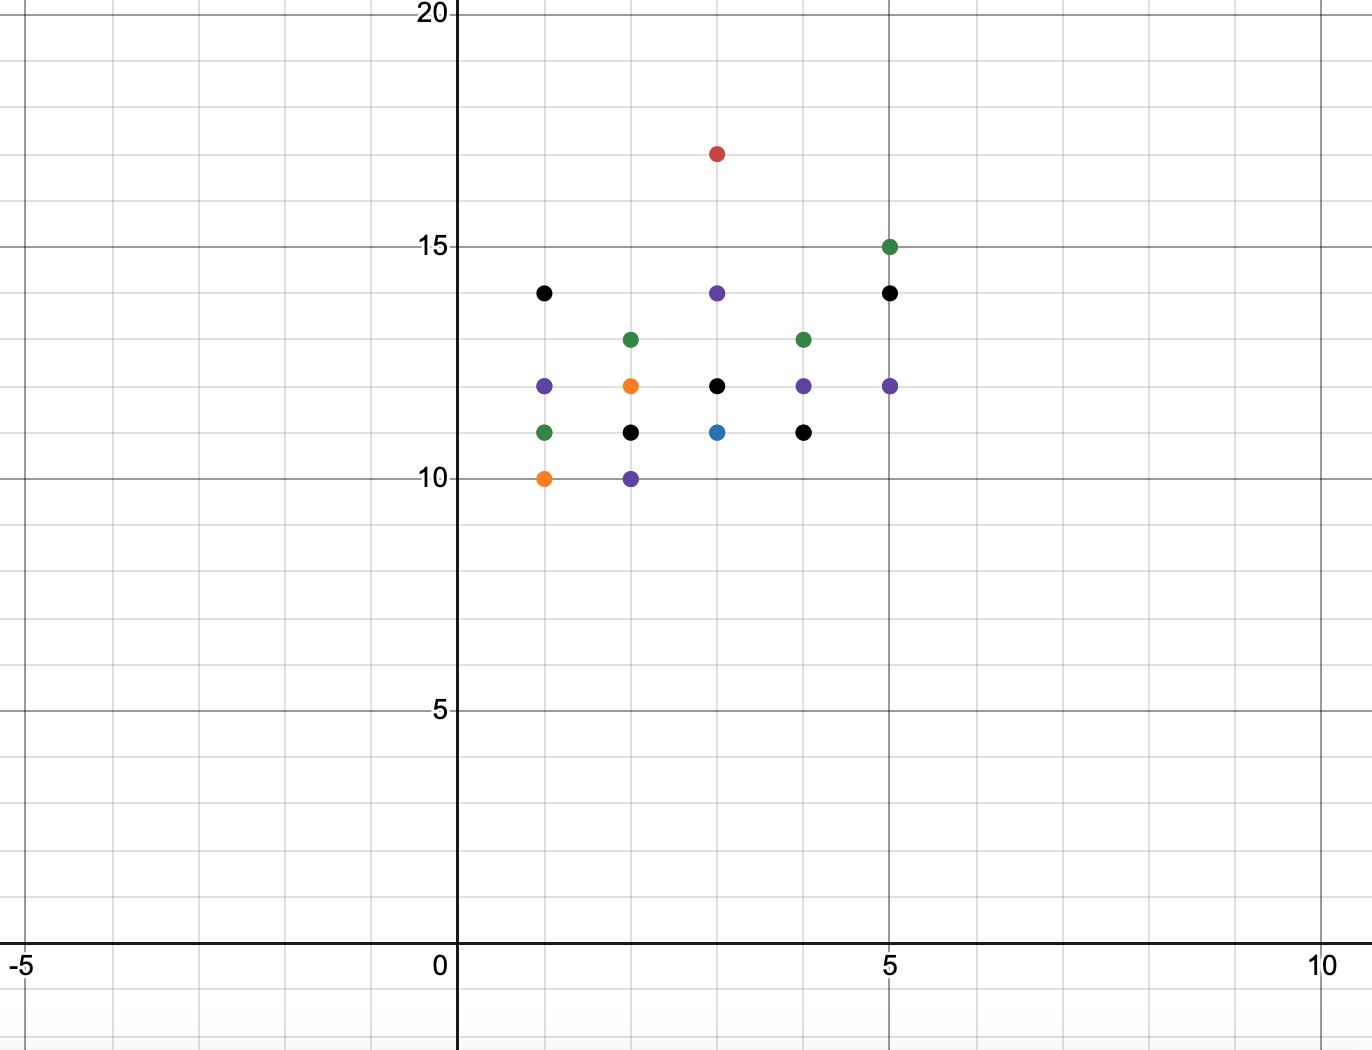
\includegraphics[width=\linewidth]{fail.png}
        \caption{First Fail}
        \label{fig:firstFail}
    \end{minipage}
    \hfill % Adds a small horizontal space between the images
    \begin{minipage}[t]{0.48\textwidth} % Second image takes up 48% of the width
        \centering
        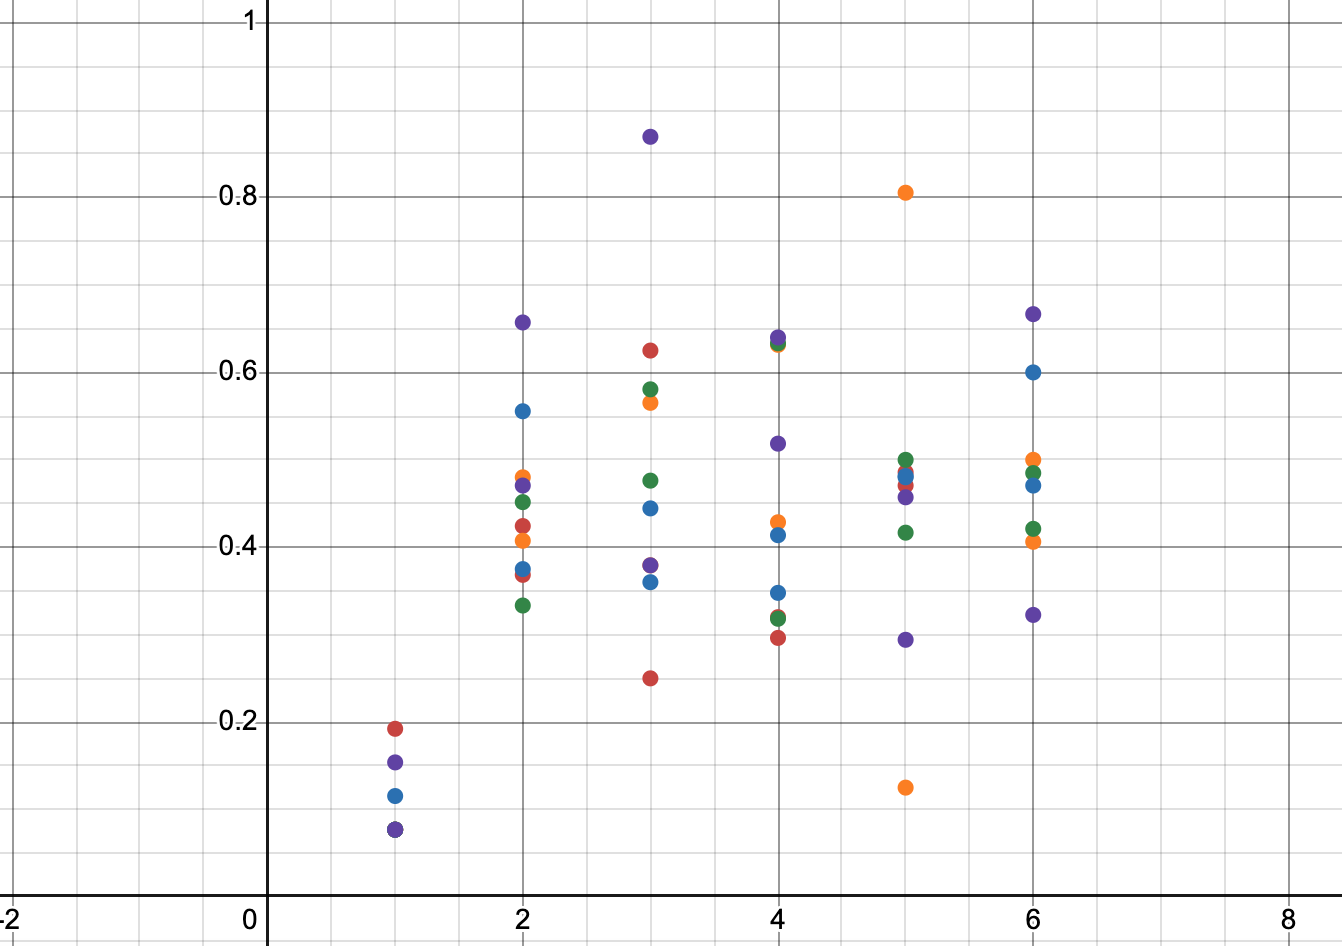
\includegraphics[width=\linewidth]{fail_pt2.png}
        \caption{Second Fail}
        \label{fig:secondFail}
    \end{minipage}
\end{figure}
 
Following this setback, I tried a different approach that still assessed the number of rounds as the independent variable, however changed the dependent variable to include the whole deck of cards. Assesssing the orderedness of the few cards faced up in front of each player could be useful for individual rounds, but the goal of assessing a whole game's progress inevitably requires analysis of the whole deck. And so, I changed the dependent variable to be the longest run that exists in each player's hand (see Table \ref{tb:variables2}), to more accurately represent the orderedness of cards as it allows for cards in order, both ascending and descending, to be recorded. 

In this new exploration, I used the following factors:

\begin{table}[H]
\centering
\begin{tabular}{lll}
\toprule
Axis & Description & Variable \\
\midrule
$x$ & The number of rounds played & Independent \\
$y$ & The length of the longest chain & Dependent \\
\bottomrule	
\end{tabular}
\caption{Variables for second investigation}
\label{tb:variables2}
\end{table}


\subsection{Data Collection}

I played 10 games of Speed, limiting each game to 5 rounds. I chose 10 as the number of games' data to collect, as the values for each round began to average out around that point (see Figure \ref{fig:10rounds1}-\ref{fig:10rounds6} below).  
 
 \begin{figure}[H]
	\begin{minipage}[t]{0.48\textwidth} % First image takes up 48% of the width
        \centering
        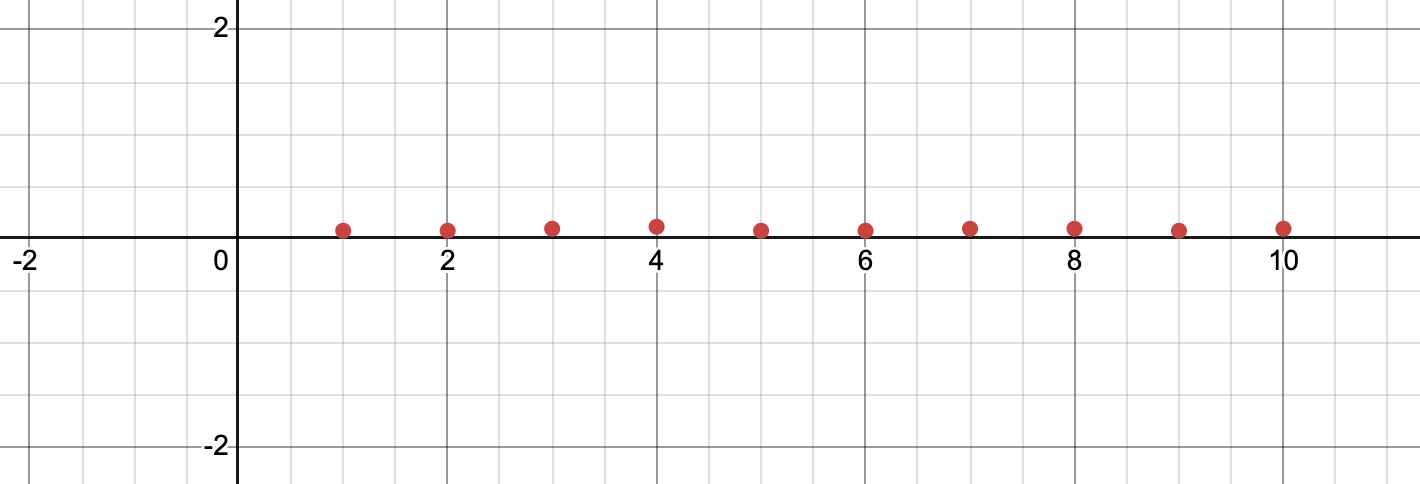
\includegraphics[width=\linewidth]{10rounds1.png}
        \caption{Round 1: graph of 10 games}
        \label{fig:10rounds1}
    \end{minipage}
    \hfill % Adds a small horizontal space between the images
    \begin{minipage}[t]{0.48\textwidth} % Second image takes up 48% of the width
        \centering
        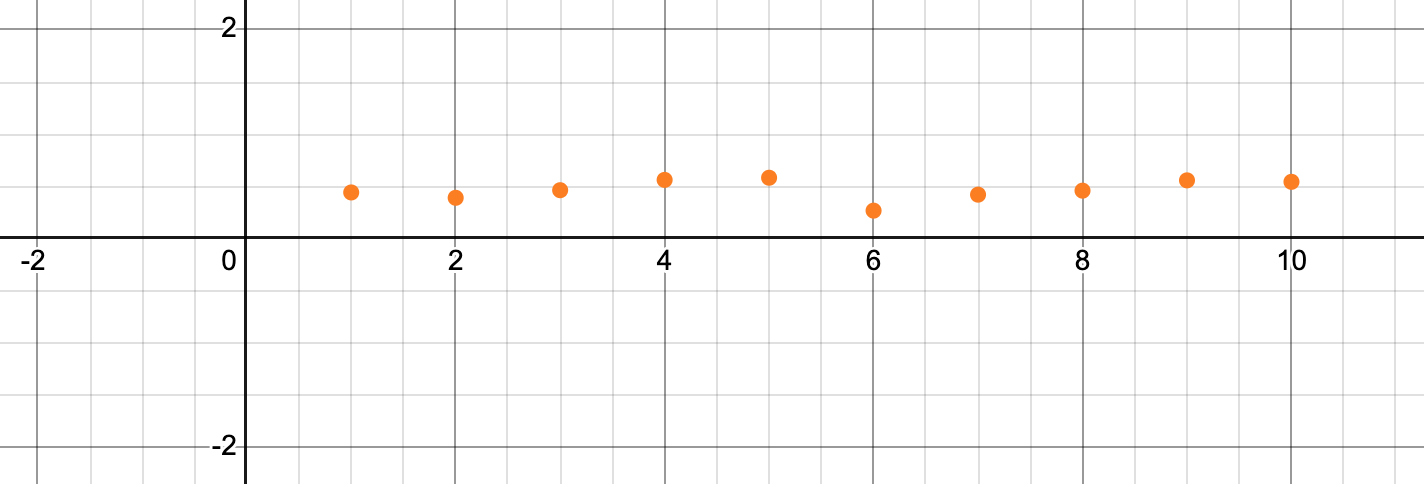
\includegraphics[width=\linewidth]{10rounds2.png}
        \caption{Round 2: graph of 10 games}
        \label{fig:10rounds2}
    \end{minipage}
\end{figure}

 \begin{figure}[H]
	\begin{minipage}[t]{0.48\textwidth} % First image takes up 48% of the width
        \centering
        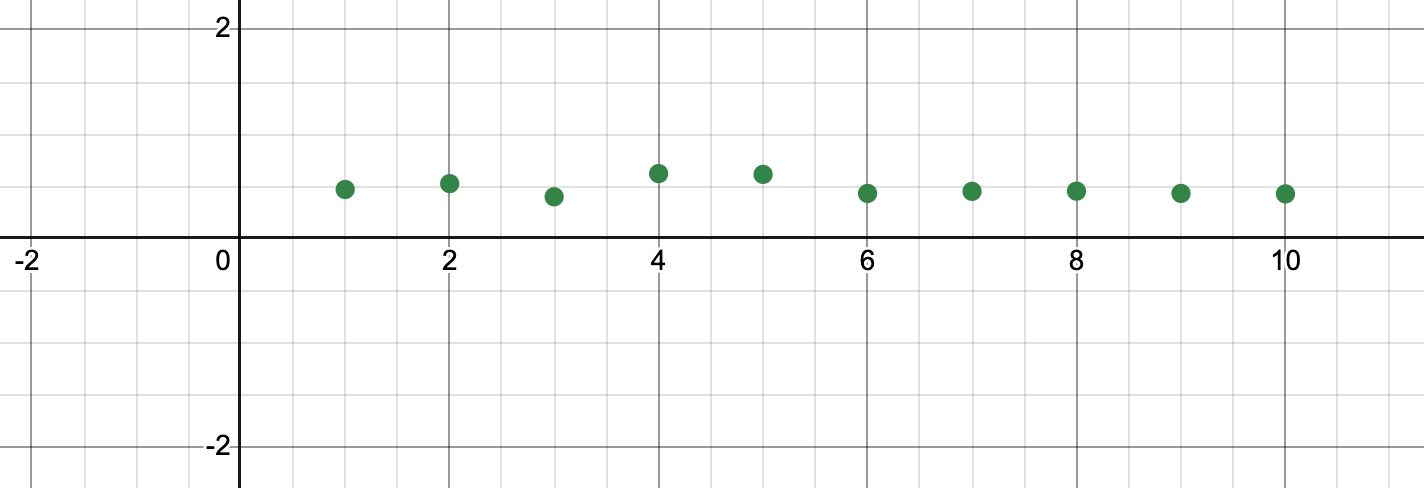
\includegraphics[width=\linewidth]{10rounds3.png}
        \caption{Round 3: graph of 10 games}
        \label{fig:10rounds3}
    \end{minipage}
    \hfill % Adds a small horizontal space between the images
    \begin{minipage}[t]{0.48\textwidth} % Second image takes up 48% of the width
        \centering
        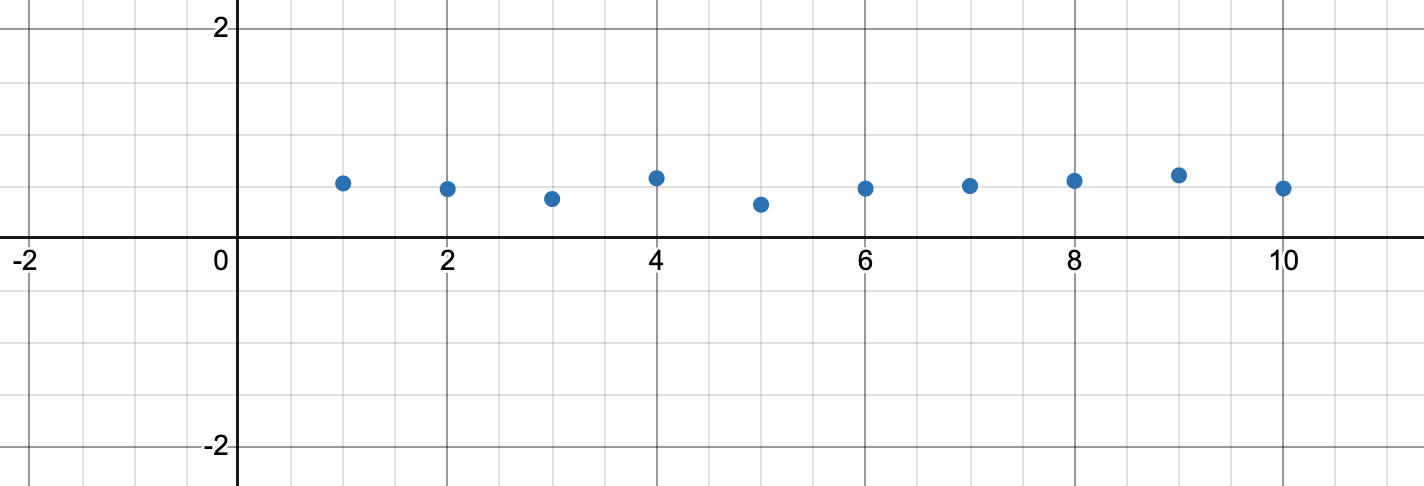
\includegraphics[width=\linewidth]{10rounds4.png}
        \caption{Round 4: graph of 10 games}
        \label{fig:10rounds4}
    \end{minipage}
\end{figure}

 \begin{figure}[H]
	\begin{minipage}[t]{0.48\textwidth} % First image takes up 48% of the width
        \centering
        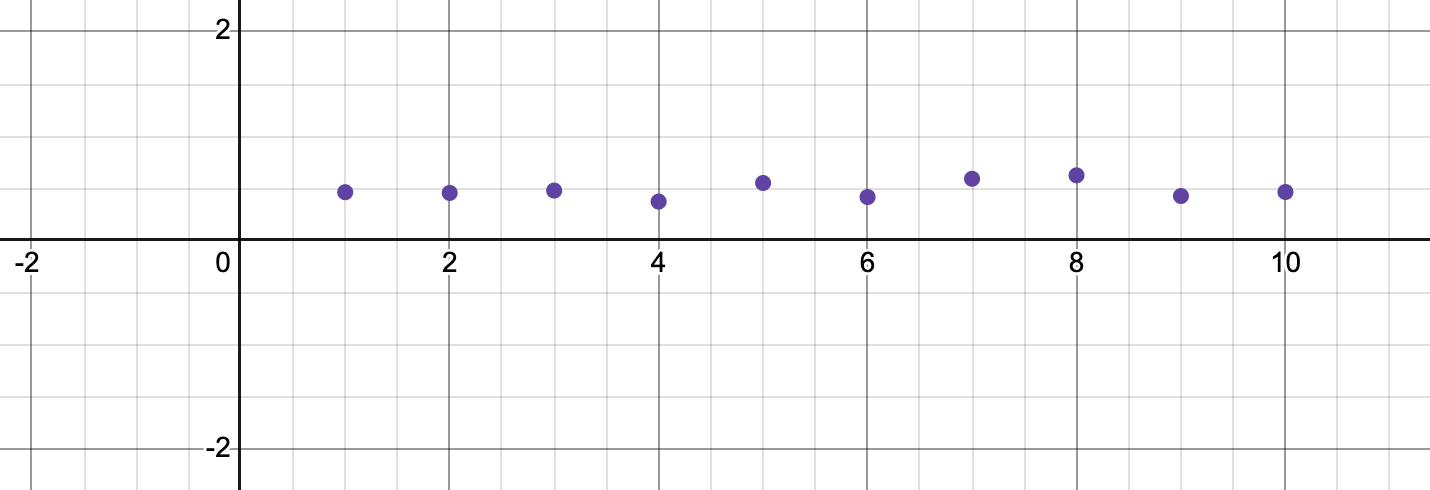
\includegraphics[width=\linewidth]{10rounds5.png}
        \caption{Round 5: graph of 10 games}
        \label{fig:10rounds5}
    \end{minipage}
    \hfill % Adds a small horizontal space between the images
    \begin{minipage}[t]{0.48\textwidth} % Second image takes up 48% of the width
        \centering
        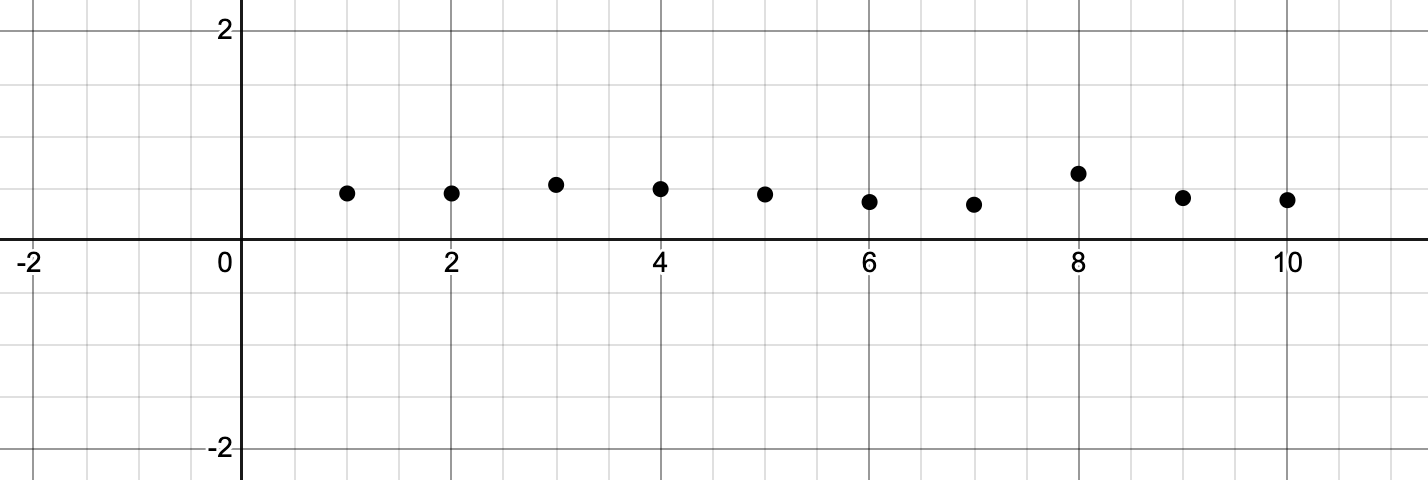
\includegraphics[width=\linewidth]{10rounds6.png}
        \caption{Round 6: graph of 10 games}
        \label{fig:10rounds6}
    \end{minipage}
\end{figure}

I took count of the $c$-value (see Definitions) before each round, and once after the final, fifth round, producing 6 data points for each game.

\begin{figure}[H]
	\centering
	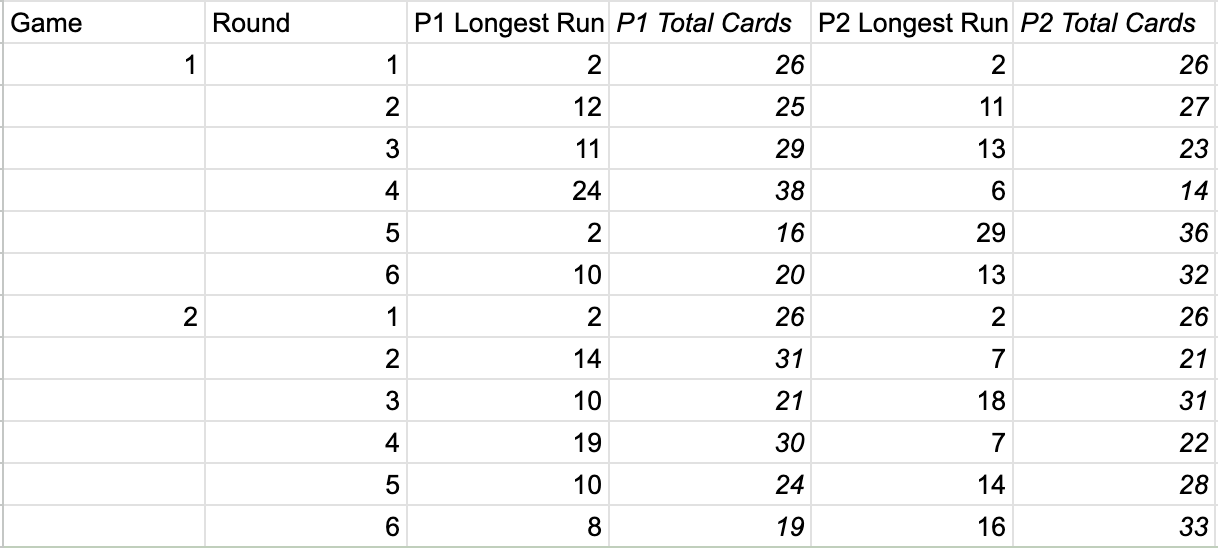
\includegraphics[scale=.5]{sample_raw_data.png}
	\caption{Table of sample raw data from game 1 and 2 (see Appendix for full raw data set)}
	\label{fig:sampleRawData}
\end{figure}

\subsection{Graphing}

After collecting adequate data on these variables, I found the average ratio (r), for each round from 0-5, for each player individually (r1 and r2), and then found the average between those, which presented the data set:

\begin{figure}[H]
	\centering
	\includegraphics[scale=.5]{sample_data.png}
	\caption{Table of sample data from game 1 and 2 (see Appendix for full raw set)}
	\label{fig:sampleData}
\end{figure}

\begin{figure}[H]
	\centering
	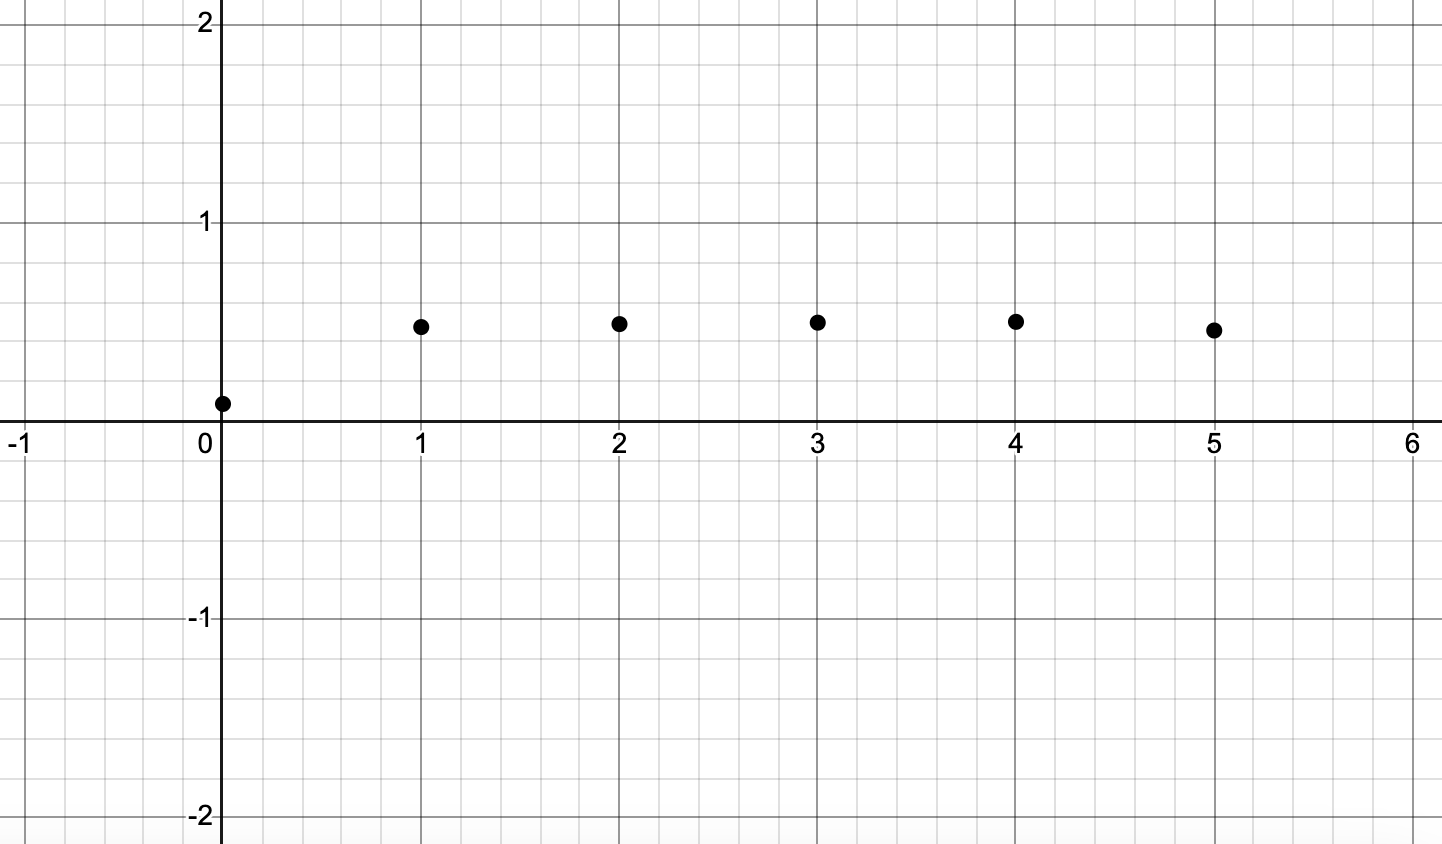
\includegraphics[scale=.4]{avg_r_value.png}
	\caption{Graph of averaged values for each round}
	\label{fig:avgRvalue}
\end{figure}

 \begin{figure}[H]
	\begin{minipage}[t]{0.48\textwidth} % First image takes up 48% of the width
        \centering
        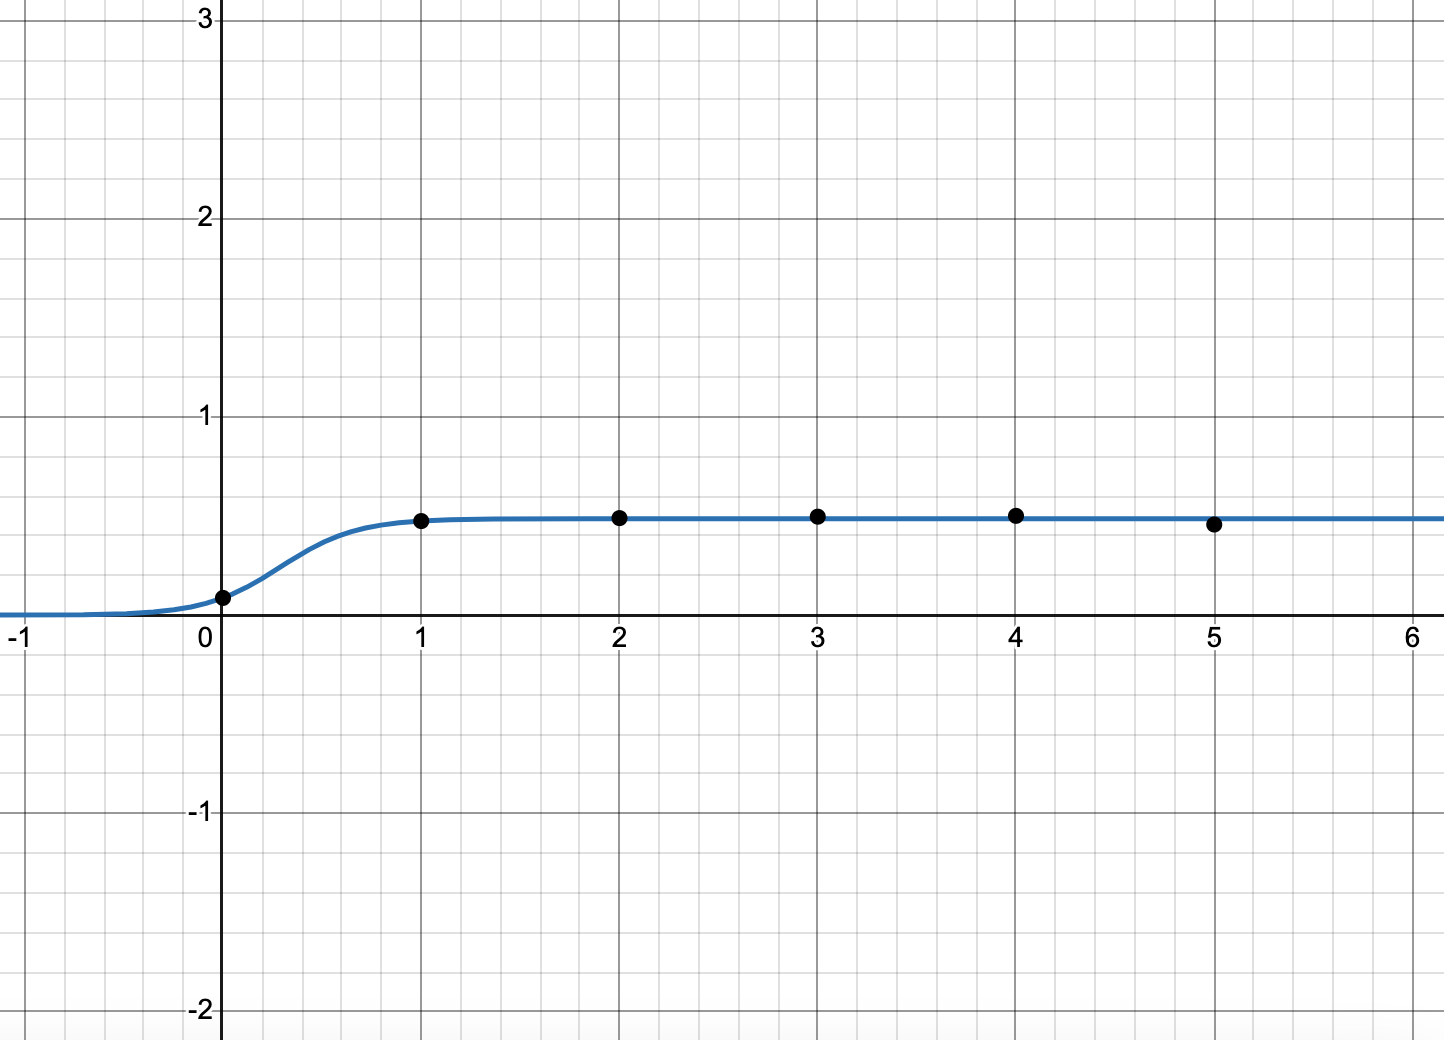
\includegraphics[width=\linewidth]{avg_r_value_logist.png}
        \caption{Graph with logistic regression line}
        \label{fig:avgRvalueLogist}
    \end{minipage}
    \hfill % Adds a small horizontal space between the images
    \begin{minipage}[t]{0.48\textwidth} % Second image takes up 48% of the width
        \centering
        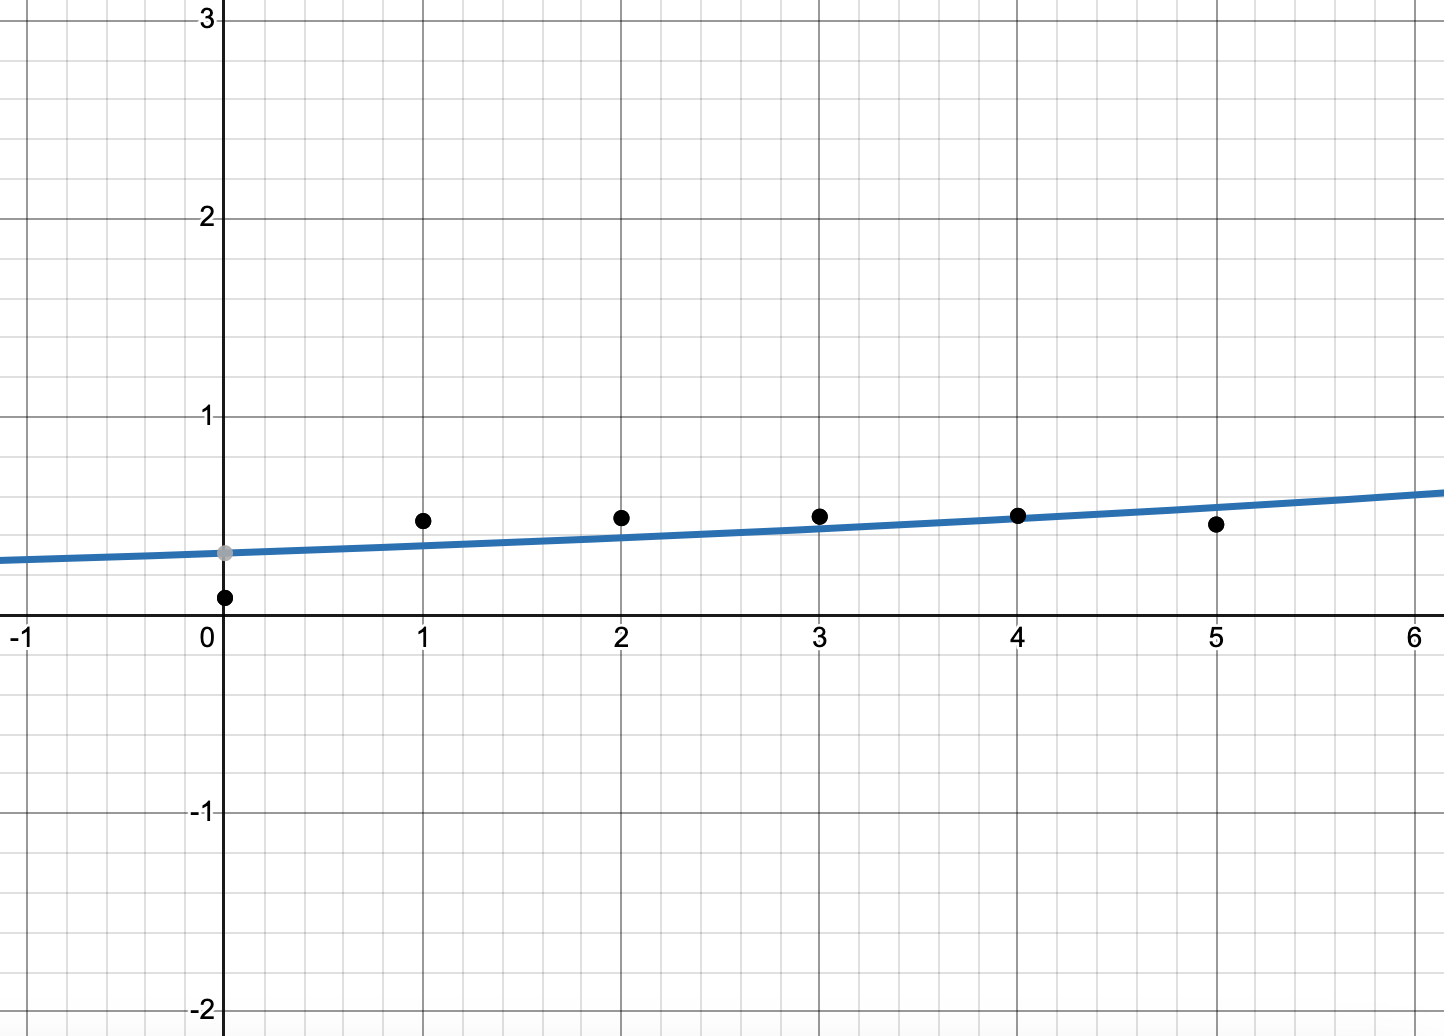
\includegraphics[width=\linewidth]{avg_r_value_expo.png}
        \caption{Graph with exponential regression line}
        \label{fig:avgRvalueExpo}
    \end{minipage}
\end{figure}

\begin{figure}[H]
	\centering
	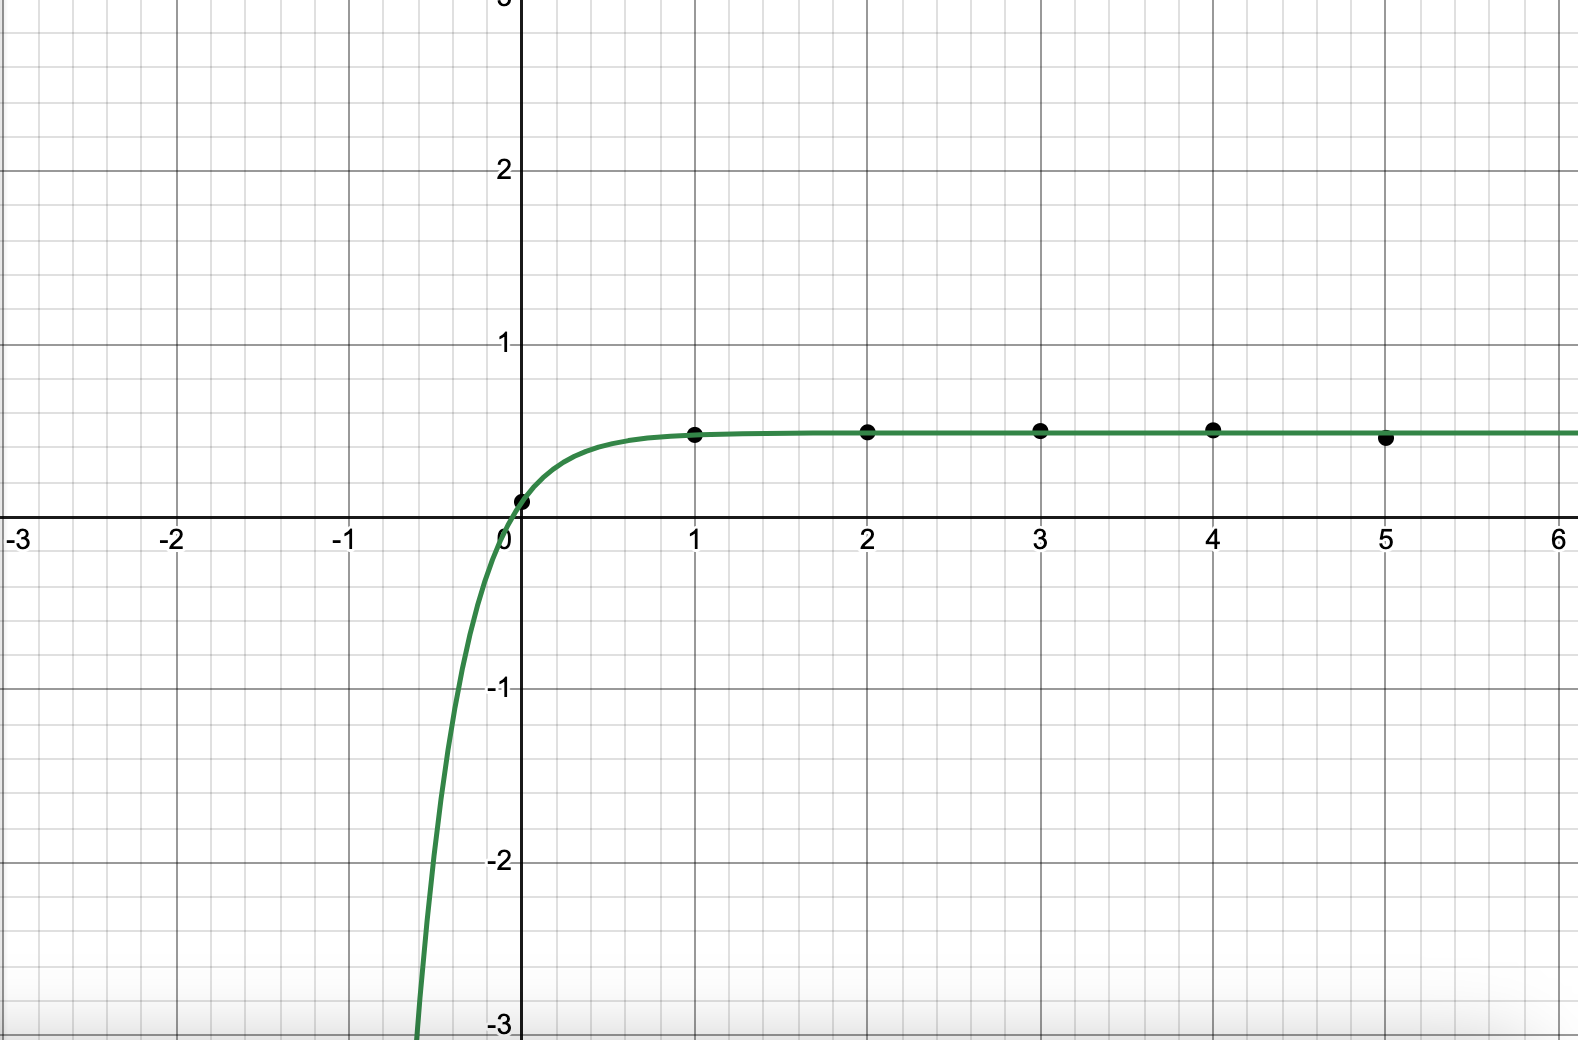
\includegraphics[scale=.5]{avg_r_value_LOBF.png}
	\caption{Graph with line of best fit}
	\label{fig:avgRvalueLOBF}
\end{figure}

%TODO fix this mistake: want to ref 2 figs
I tried various regression lines on this data (Figure \ref{fig:avgRvalueLogist} \ref{fig:avgRvalueExpo}), however evidently the line of best fit was the exponential graph (\ref{fig:avgRvalueLOBF}) with the following equation:

\begin{equation}
	y={a\cdot{b}^{cx}+d}
	\label{eq:expFormula	}
\end{equation}



With the following values:

$a$=-0.399228  \\
$b$=0.150864 \\
$c$=1.8832 \\
$d$=0.486637 \\

Where b and c can be grouped together, and d is expected to act as an asymptote however

The average orderliness at the start ($x=0$), prior to any game-playing can be derived through algebra:

\begin{equation}
y={a\cdot{b}^{cx}+d} \\
y=a+d \\
y=-0.399228+0.486637 \\
y=0.087409 \\
\label{initialOrder}	
\end{equation}

The average orderliness at the end ($x=5$), following the 5th round of game-playing can also be derived through algebra:

\begin{equation}
y={a\cdot{b}^{cx}+d}
y={-0.399228\cdot{0.150864}^{1.8832\cdot{5}}+0.486637}
y=
y=0.087409
\label{initialOrder}	
\end{equation}



This graph illustrates the extreme incline and then rounding and ultimately flat-lining of the data best, especially in comparison to the others. This curve also begins by going directly up, rather than gradually ascending, such as in Fig. 13.
From this graph, we learn that the relationship between the number of rounds played and the number of cards in the longest chain is weak in the first round, however thereafter increases sharply and settles around 0.45-0.5 without dramatically increasing or decreasing, indicating n asymptotic nature of the orderedness of cards in Speed rounds. Through a real-world lens, this ultimately indicates that while the more rounds played does result in more ordered cards, this does not perpetuate the cycle entirely until the entire deck is ordered, but rather cuts off once the deck reaches a certain level of orderedness.


to do 
avg orderliness at the stratr using algerba
avg. end asymptote orderliness using algebra
what is avg extra it gets each time (round)
assumption: exponential, got evidence
use AI to make suggestion about maths to research

find a and d

a+d= y-int (initial orderliness)
d: end-point ordelriness

b: how ordered is the pile

- look at textbook for stats



